\begin{figure}[!htbp]
\begin{center}
    % \vspace{-1em}
    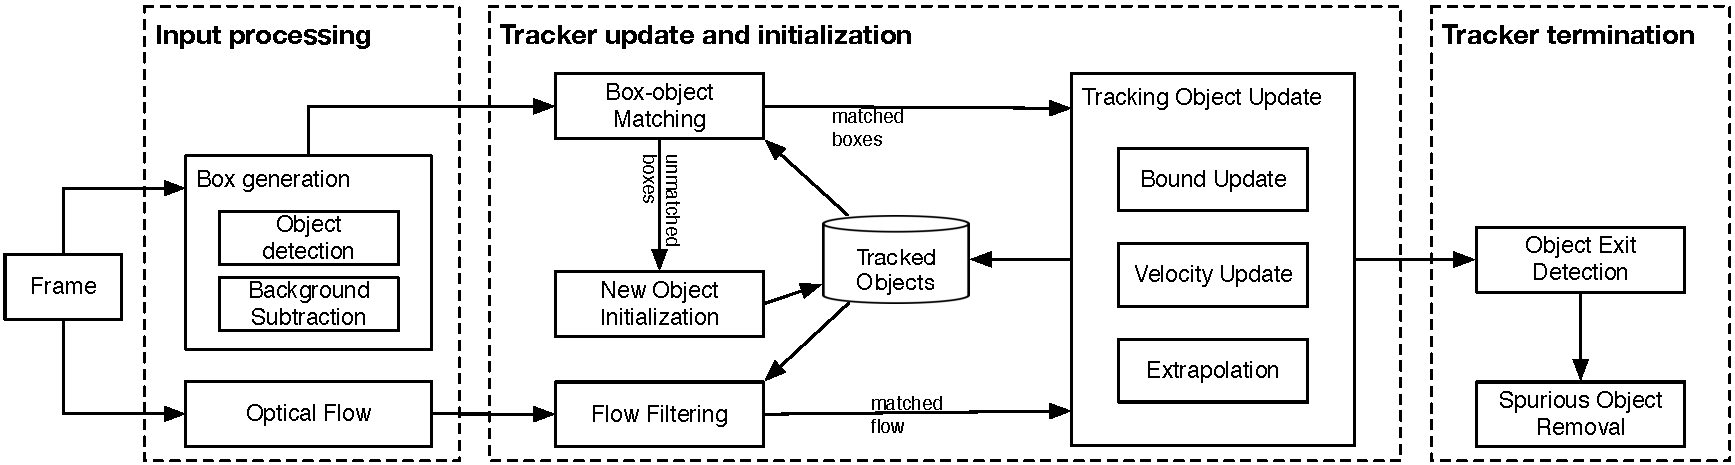
\includegraphics[width=\linewidth]{./img/kalmanFilterTracker.pdf}
\end{center}
    % \vspace{-1em}
   \caption{Overview of proposed system. Separate Kalman filter state is initialized, maintained and terminated for each tracked object. The state is updated based on matching input from background subtraction, object detection and optical flow.}
\label{fig:kf-tracker-workflow}
% \vspace{-1em}
\end{figure}